\documentclass{beamer}
\usepackage[utf8]{inputenc}
\usepackage{graphicx}
\usepackage{xspace} % Needed for macro \xspace

% Remove navigation controls
\usenavigationsymbolstemplate{}

% Slide numbering
\setbeamertemplate{footline}[frame number]

% Convienence macro
\newcommand{\atweb}{\textbf{@Web}\xspace}

% Macro for writing an RDF triplet
\newcommand{\triplet}[1]{$\langle$\texttt{#1}$\rangle$}

\title{An introduction to the semantic web technologies}
\subtitle{
  And their use within the \atweb platform
}
\author{
  Leandro Lovisolo
}
\date{September 23, 2015}
\institute{
  INRA SupAgro and INRIA GraphiK \\
  Montpellier, France
}

\begin{document}

\begin{frame}
  \titlepage
\end{frame}

\begin{frame}
  \frametitle{Outline of the presentation}

  \begin{itemize}
    \item What's an ontology?
    \item RDF
    \item RDFS
    \item OWL
    \item SKOS
    \item SPARQL
    \item The n-ary relationship pattern used in \atweb
    \item Examples of tables in scientific documents annotated using n-ary
      relationships in \atweb
  \end{itemize}
\end{frame}

\begin{frame}
  \frametitle{What's an ontology?}

  \pause

  It's a formal description of a domain of interest based on:

  \pause

  \begin{itemize}
    \item a set of \textit{individuals} (also called entities or objects),

    \pause

    \item a set of \textit{classes} of individuals, and

    \pause

    \item a set of \textit{relationships} (sometimes called properties)
      between these individuals;
  \end{itemize}

  \pause

  and a set of logical constraints to specify, among other things:

  \pause

  \begin{itemize}
    \item class membership,

    \pause

    \item subclass/subproperty relationships,

    \pause

    \item domain/range restrictions on properties,

    \pause

    \item cardinality constraints,

    \pause

    \item class union/intersection/disjointness constraints,

    \pause

    \item etc.
  \end{itemize}
\end{frame}

\begin{frame}
  \frametitle{Web resources, URI, namespaces}

  \pause

  A \textit{resource} is anything that can be referred to: a web page, a
  person, a city, a university course, etc.

  \pause

  \medskip

  Resources are identified by \textit{URIs}, for example:

  \begin{itemize}
    \item \texttt{http://example.com/MyOntology},
    \item \texttt{http://example.com/MyOntology\#Leandro},
    \item \texttt{http://example.com/MyOntology\#Pizza},
    \item etc.
  \end{itemize}

  \pause

  To avoid carrying long URIs, \textit{namespaces} are used. \pause Thus,

  \pause

  \begin{itemize}
    \item \texttt{http://example.com/MyOntology} \pause \hfill becomes

    \pause

    \item \texttt{example:MyOntology} \pause \hfill abbreviated as

    \pause

    \item \texttt{:MyOntology}
  \end{itemize}

  \pause

  if \texttt{example} is the default namespace.
\end{frame}

\begin{frame}
  \frametitle{RDF}

  A simple language for describing \textit{annotations} about Web resources
  identified by URIs, from now on referred to as \textbf{facts}.
\end{frame}

\begin{frame}
  \frametitle{RDF}
  \framesubtitle{Triplets}

  Facts are stated as \textit{RDF triplets}.

  \pause

  \medskip

  A triplet is made of a \textit{subject}, an \textit{object} and a
  \textit{predicate}.

  \pause

  \medskip

  Some examples:

  \pause

  \begin{itemize}
    \item \triplet{:Dupond :Leads :InfoDept}

    \pause

    \item \triplet{:Dupond :TeachesIn :UE111}

    \pause

    \item \triplet{:Dupond :TeachesTo :Pierre}

    \pause

    \item \triplet{:Pierre :EnrolledIn :InfoDept}

    \pause

    \item \triplet{:Pierre :RegisteredTo :UE111}

    \pause

    \item \triplet{:UE111 :OfferedBy :InfoDept}
  \end{itemize}
\end{frame}

\begin{frame}
  \frametitle{RDF}
  \framesubtitle{Graph representation}

  \begin{center}
    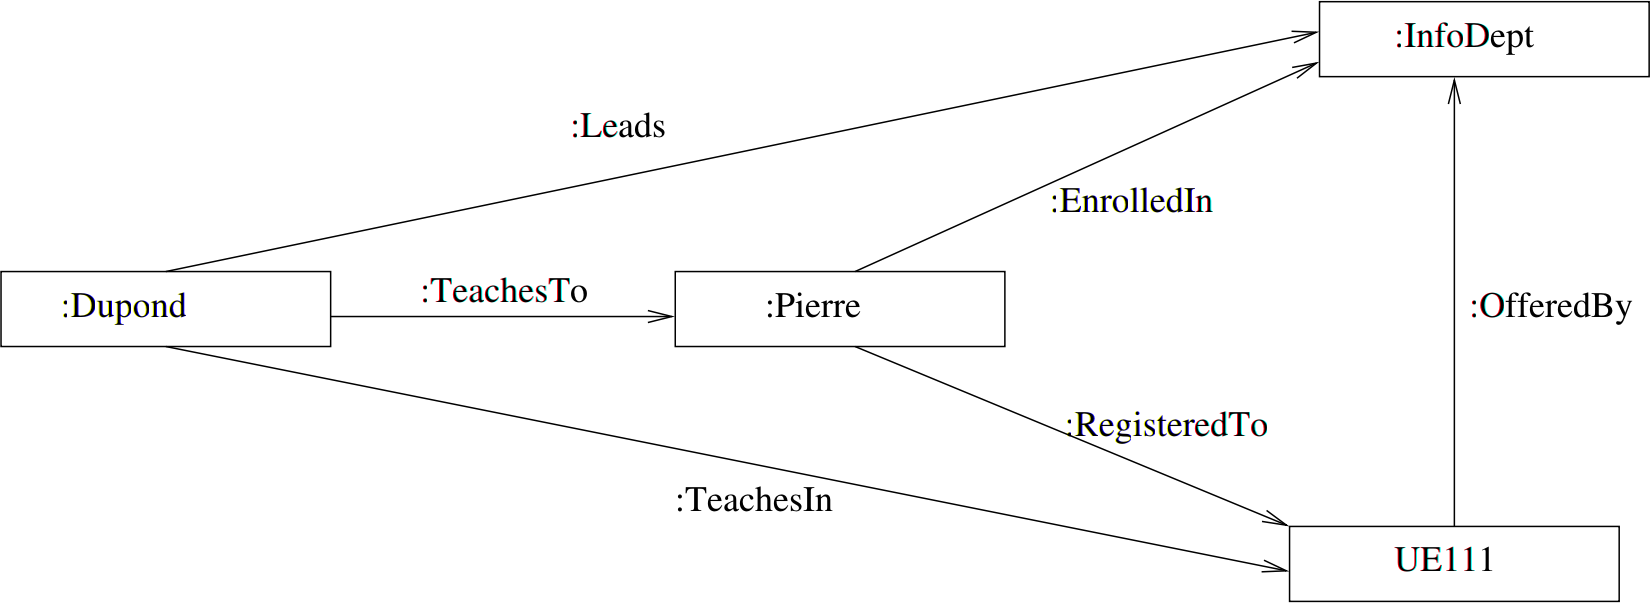
\includegraphics[width=11cm]{graph.png}
  \end{center}

  \triplet{:Dupond :Leads :InfoDept} \\
  \triplet{:Dupond :TeachesIn :UE111} \\
  \triplet{:Dupond :TeachesTo :Pierre} \\
  \triplet{:Pierre :EnrolledIn :InfoDept} \\
  \triplet{:Pierre :RegisteredTo :UE111} \\
  \triplet{:UE110 :OfferedBy :InfoDept}
\end{frame}

\begin{frame}
  \frametitle{RDF}
  \framesubtitle{Syntax}

  There are many different syntaxes for writing RDF triplets, including:

  \pause

  \begin{itemize}
    \item XML (as used in \atweb),

    \pause

    \item Turtle,
    \item N-Triples,
    \item N-Quads,
    \item etc.
  \end{itemize}

  \pause

  However, we're going to focus on the abstract \triplet{subject, predicate,
  object} syntax during this presentation.
\end{frame}

\begin{frame}
  \frametitle{}
\end{frame}

\begin{frame}
  \frametitle{}
\end{frame}

\begin{frame}
  \frametitle{}
\end{frame}

\begin{frame}
  \frametitle{}
\end{frame}

\begin{frame}
  \frametitle{}
\end{frame}

\begin{frame}
  \frametitle{Motivation}
  \framesubtitle{Problem statement}

  \pause

  \begin{itemize}
    \item We're trying to answer questions that require consulting
      heterogeneous data sources.

    \pause

    \begin{itemize}
      \item Literature with inconsistent, semi-structured data.

      \pause

      \item No standard naming convention.

      \pause

      \item No information about the reliability of the data sources.

      \pause

      \item Each data source has its specific browsing/querying mechanism (no
        common interface.)
    \end{itemize}
  \end{itemize}
\end{frame}

\begin{frame}
  \frametitle{Motivation}
  \framesubtitle{Sample problem domain: \textbf{biorefinery}}

  \begin{itemize}
    \item Ligno-cellulosic biomass pre-treatment before enzymatic hydrolysis is
      an essential step to obtain good yields.

    \pause

    \item Several pre-treatment principles available, but \textbf{no clear
      criteria on how to choose the best one} taking into account environmental
      sustainability for a given biomass and biorefinery product (e.g.
      glucose.)
  \end{itemize}
\end{frame}

\begin{frame}
  \frametitle{Proposed solution}

  \begin{itemize}
    \item Represent scientific knowledge with ontologies using recommended
      standardized tools and languages for such purposes (semantic web
      technologies, RDF(S), OWL, etc.)

    \pause

    \item Develop an ontology and data management web application (e.g. the
      \textbf{@Web platform}) that makes it easy for scientists to introduce
      data from scientific publications into an ontology, execute queries
      against an ontology, etc.

    \pause

    \item Create integrity constraints to automatically detect inconsistencies
      and errors in scientific publications and to automatically classify
      publications according to their topics.

    \pause

    \begin{itemize}
      \item \textit{The focus of my internship!}
    \end{itemize}

  \end{itemize}
\end{frame}

\begin{frame}
  \frametitle{An example of a termino-ontological resource}
  \framesubtitle{Taken from the biorefinery application}

  \begin{center}
    % 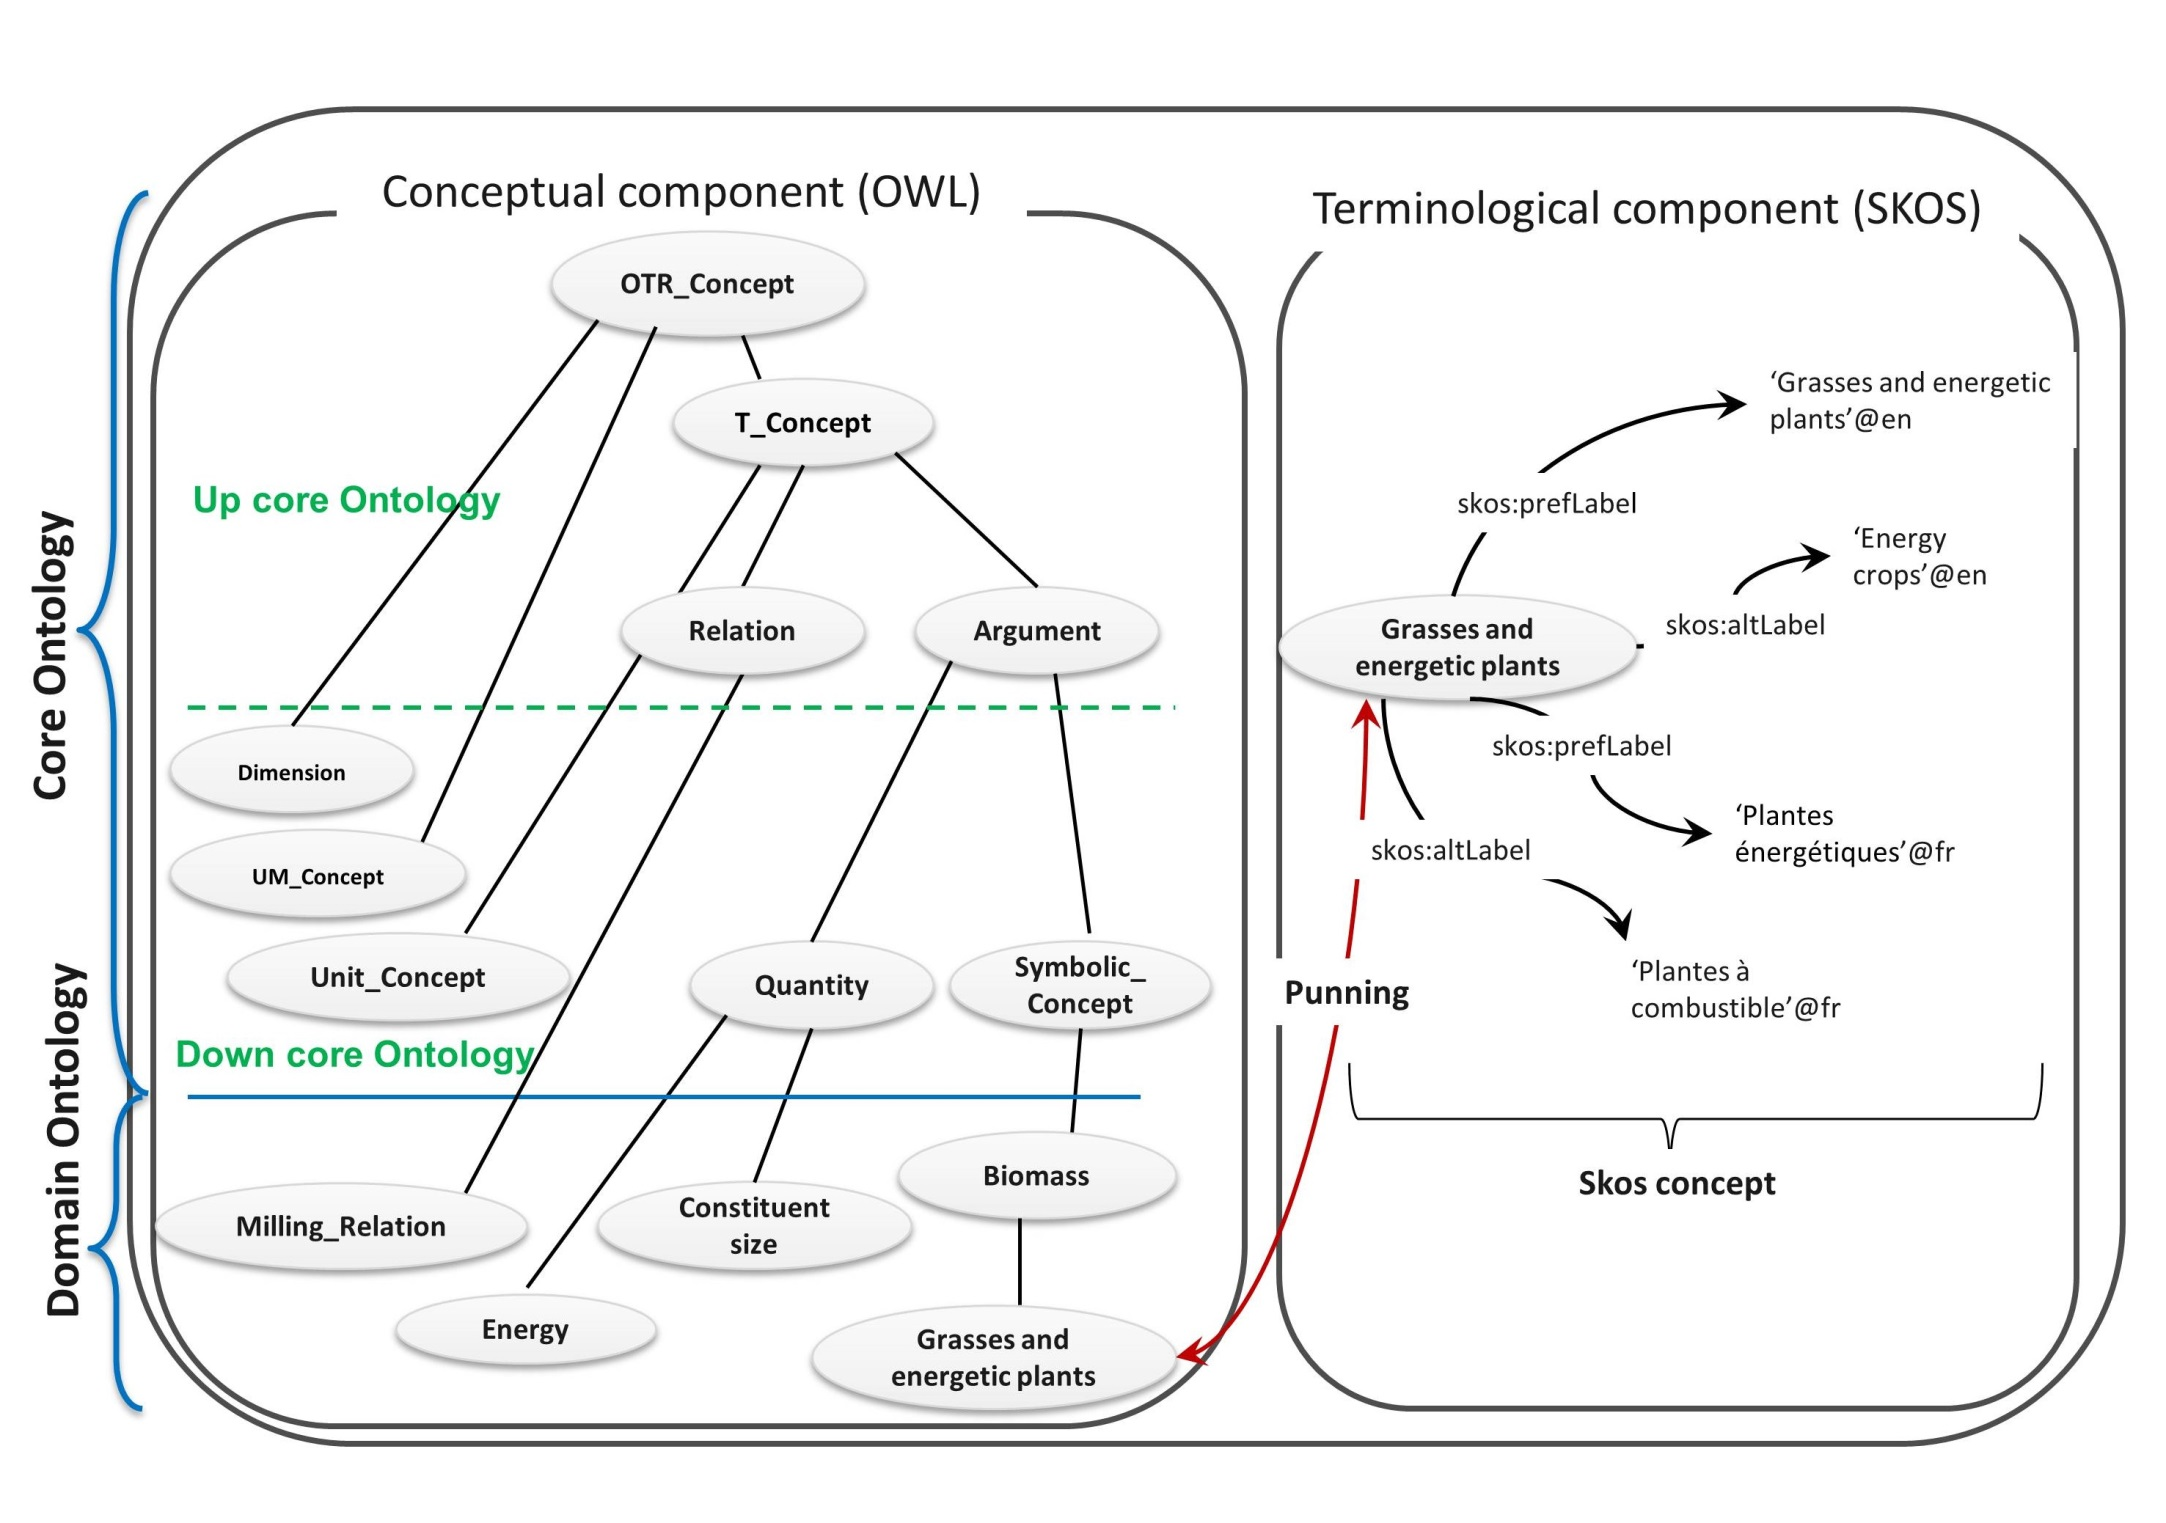
\includegraphics[width=10cm]{termino-ontological-resource.jpg}
  \end{center}
\end{frame}

\begin{frame}
  \frametitle{Design goals for the core ontology}

  \begin{itemize}
    \item \textbf{Simple} so as to make the annotator's task easier.

    \pause

    \item \textbf{Generic} enough so that the approach can be applied to
      different, unrelated domains.

    \pause

    \begin{itemize}
      \item Proven in the domains of biorefinery and packaging selection.
    \end{itemize}
  \end{itemize}
\end{frame}

\begin{frame}
  \frametitle{A sample relation}
  \framesubtitle{Also from the biorefinery domain}

  \begin{center}
    % 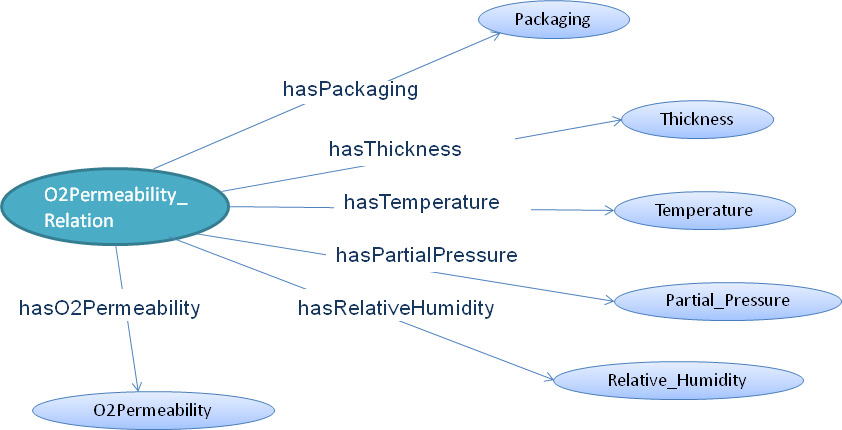
\includegraphics[width=10cm]{relation.jpg}
  \end{center}
\end{frame}

\begin{frame}
  \frametitle{The \textbf{@Web} platform}
  \framesubtitle{Exploring an ontology}

  \begin{center}
    % \includegraphics[width=8cm]{atweb-ontology.jpg}
  \end{center}
\end{frame}

\begin{frame}
  \frametitle{The \textbf{@Web} platform}
  \framesubtitle{Browsing documents}

  \begin{center}
    % \includegraphics[width=10cm]{atweb-document.jpg}
  \end{center}
\end{frame}

\begin{frame}
  \frametitle{The \textbf{@Web} platform}
  \framesubtitle{Querying an ontology: defining the search scope}

  \begin{center}
    % \includegraphics[width=10cm]{atweb-query-1.jpg}
  \end{center}
\end{frame}

\begin{frame}
  \frametitle{The \textbf{@Web} platform}
  \framesubtitle{Querying an ontology: search parameters}

  \begin{center}
    % \includegraphics[width=10cm]{atweb-query-2.jpg}
  \end{center}
\end{frame}

\begin{frame}
  \frametitle{The \textbf{@Web} platform}
  \framesubtitle{Querying an ontology: executing a query}

  \begin{center}
    % \includegraphics[width=10cm]{atweb-query-3.jpg}
  \end{center}
\end{frame}

\begin{frame}
  \frametitle{The \textbf{@Web} platform}
  \framesubtitle{Querying an ontology: results}

  \begin{center}
    % \includegraphics[width=10cm]{atweb-query-4.jpg}
  \end{center}
\end{frame}

\begin{frame}
  \frametitle{The annotator's task}

  \begin{itemize}
    \item Given a scientific publication and a desired ontology, capture data
      from the publication using the appropriate concepts in the ontology.

    \pause

    \item Create and update concepts in the ontology as they're discovered
      during the annotation process (i.e. in an iterative fashion.)

    \pause

    \item Write and edit \textbf{guidelines} associated to each concept
      explaining when and how a concept should be used.
  \end{itemize}
\end{frame}

\begin{frame}
  \frametitle{An example of data captured from a scientific publication}

  \begin{center}
    % 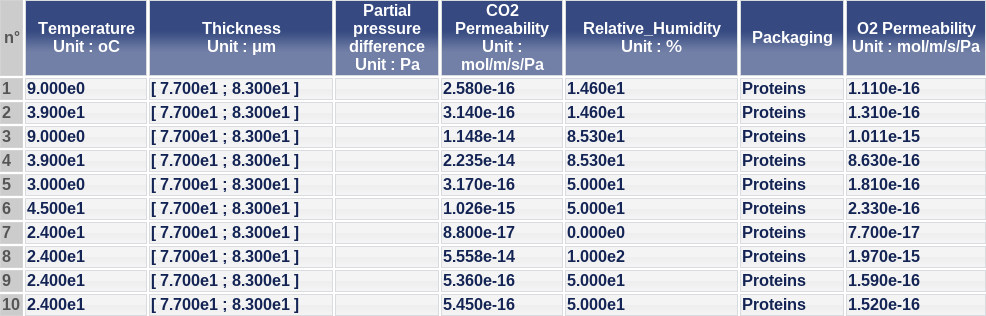
\includegraphics[width=11cm]{table.jpg}
  \end{center}
\end{frame}

\begin{frame}
  \frametitle{A sample guideline}

  \begin{center}
    % \includegraphics[width=10cm]{guideline.jpg}
  \end{center}
\end{frame}

\begin{frame}
  \frametitle{Some sample guidelines that can be easily translated into SPARQL
  constraints}
  \framesubtitle{Integrity constraints}

  \begin{itemize}
    \item \textit{``The output quantity of a step is equal to the sum of the
      quantity of water used and the quantity of biomass present in the
    step.''}

    \pause

    \item \textit{``The second milling step must give an “Output solid
      constituent size” smaller than 0,5-1 mm.''}
  \end{itemize}
\end{frame}

\begin{frame}
  \frametitle{Some sample guidelines that can be easily translated into SPARQL
  constraints}
  \framesubtitle{Classification constraints}

  \begin{itemize}
    \item \textit{``Topic Bioref-PM-PC-UFM-PS : included experiments are
      composed of a pre-milling step, followed by a physico-chemical treatment,
    then by an ultrafine milling step (ball milling, wet disk milling, etc.), a
  press and separation step (washing and filtration), and finally the enzymatic
hydrolysis step. This topic requires a press and separation step because there
are a lot of effluents in the physico-chemical step or because the milling is
made with effluent. The second milling step must give an “Output solid
constituent size” smaller than 0,5-1 mm. (en)''}
  \end{itemize}
\end{frame}

\begin{frame}
  \frametitle{Examples of guidelines that \textbf{cannot} be easily
  translated into SPARQL constraints}

  \begin{itemize}
    \item \textit{``In all treatments, when the authors indicate ``overnight'',
      we considered a duration treatment between 10 and 15 hours''}

    \pause

    \item \textit{``Furthermore, we consider that the glucose rate equals to
      glucan rate divided by 0.9.''}
  \end{itemize}
\end{frame}

\begin{frame}
  \frametitle{Statistics}
  \framesubtitle{A promising approach}

  In the biorefinery ontology alone we have:

  \begin{itemize}
    \item 11 occurrences of the phrase \textit{``equal to''}
    \item 5 occurrences of the phrase \textit{``equals to''}
    \item 11 occurrences of the phrase \textit{``sum of''}
    \item 3 occurrences of the phrase \textit{``divided by''}
    \item 2 occurrences of the phrase \textit{``multiplied by''}
  \end{itemize}

  spread across guidelines associated with 30 relation concepts.

  \vspace{1em}

  \textbf{At least 10 of them can be easily translated into SPARQL constraints.}
\end{frame}

\begin{frame}
  \begin{center}
    \Huge{Thanks!}
  \end{center}
\end{frame}

\end{document}
